% Needs Package: 
%\usepackage{bm}
%\usepackage{multicol}
\section{LTI-Systeme}

$ y(t) = \mathcal{T}[x(t)]$

\begin{multicols}{2}
    \subsection*{Linearität und Zeitinvarianz}
    \begin{itemize}
        \item $\mathcal{T}[x_1(t) + x_2(t)] = y_1(t) + y_2(t)$
        \item $\mathcal{T}[k_a \cdot x(t)] = k_a \cdot y(t)$
        \item $\mathcal{T}[x(t-t_0) = y(t-t_0)]$
    \end{itemize}

    \subsection{Beschreibung von LTI Systemen}

    \subsubsection{Impulsantwort}
    Impulsfunktion $\delta(t)$ wird am Eingang des Systems angelegt,
    die Reaktion darauf am Ausgang nennt man die \textbf{Impulsantwort} \bm{$h(t)$}.
    Sie beschreibt ein LTI-System vollständig.

    $$ y(t) = \mathcal{T}[x(t)]
        = \int \limits _{-\infty} ^{\infty} x(\tau) \cdot h(t-\tau)d\tau
        = x(t) * h(t)$$
  
    \subsubsection{Frequenzantwort}
    Die \textbf{Frequenzantwort} $\bm{H(\omega)}$ ist die Fouriertransformierte Impulsantwort.
    Sie ist eine komplexwertige dimensionslose Gewichstsfunktion.
    Auch sie beschreibt ein LTI-System vollständig.

    $$ Y(\omega) = X(\omega) \cdot H(\omega)$$

    \subsubsection{Berechnung des Ausgangssignals}
\begin{enumerate}
   \item Fourier-Transformation:  $X(\omega) = \mathcal{F}[x(t)]$ 
   \item Berechnung in Frequenz  $Y(\omega) = X(\omega) \cdot H(\omega)$ 
   \item Rücktransformation:  $y(t) = \mathcal{F}^{-1}[Y(\omega)]$ 
\end{enumerate}


    \subsection{Bezeichnungen}
    Übertragungsfunktion: $H(\omega)=|H(\omega)| \cdot e^{j\varphi_H(\omega)}$ \\
    Amplitudengang: $|H(\omega)|$ \\
    Phasengang: $\varphi_H(\omega)$ \\

    \subsubsection{Filtereigenschaften}
    $Y(\omega) = X(\omega) \cdot H(\omega)$ \\
    $|Y(\omega)| = |X(\omega)| \cdot |H(\omega)|$ \\
    $\varphi_y(\omega) = \varphi_x(\omega) + \varphi_H(\varphi)$

    \subsection{BIBO-Stabilität}
    Ein LTI-System ist genau dann BIBO-stabil, wenn die Konvergenzhalbebene seiner Übertragungsfunktion G = G(s) die imaginäre Achse (also die jω-Achse) enthält.
Das wiederum ist dann der Fall, wenn alle Polstellen sp der Übertragungsfunktion links von
der imaginären Achse liegen, d.h. wenn jeweils Re(sp) < 0.
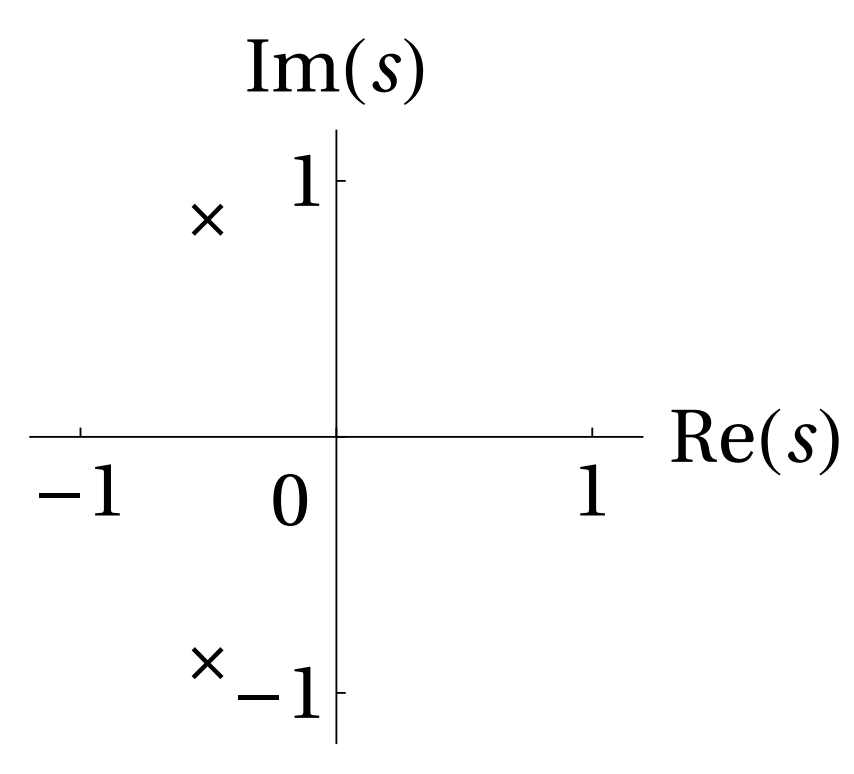
\includegraphics[width = 3cm]{include/Integraltransformationen/img/BiBo.png}

\end{multicols}
